\documentclass{beamer}

\graphicspath{{./Bilder/},{../Session_1/Bilder}}
\usepackage{blindtext}
\usepackage{booktabs}

\title{Quanten und Photonen}
\subtitle{Eine Einführung}

\author{Uwe Ziegenhagen}
\institute{DLR}

\begin{document}

\begin{frame}
\maketitle
\end{frame}

\begin{frame}[allowframebreaks]
\frametitle{Hallo DLR}
\framesubtitle{Beamer ist toll}

\blindtext[2]

\end{frame}

\begin{frame}
\frametitle{Aufzählungen}

\begin{itemize}
\item Hallo
\item ich 
\item bin 
\item eine 
\item Aufzählungsliste
\item Hallo Welt
\end{itemize}
\end{frame}

\begin{frame}
\frametitle{Aufzählungen}

\begin{enumerate}[I]
\item Hallo
\item ich 
\item bin 
\item eine 
\item Aufzählungsliste
\item Hallo Welt
\end{enumerate}
\end{frame}

\begin{frame}
\frametitle{Bilder}

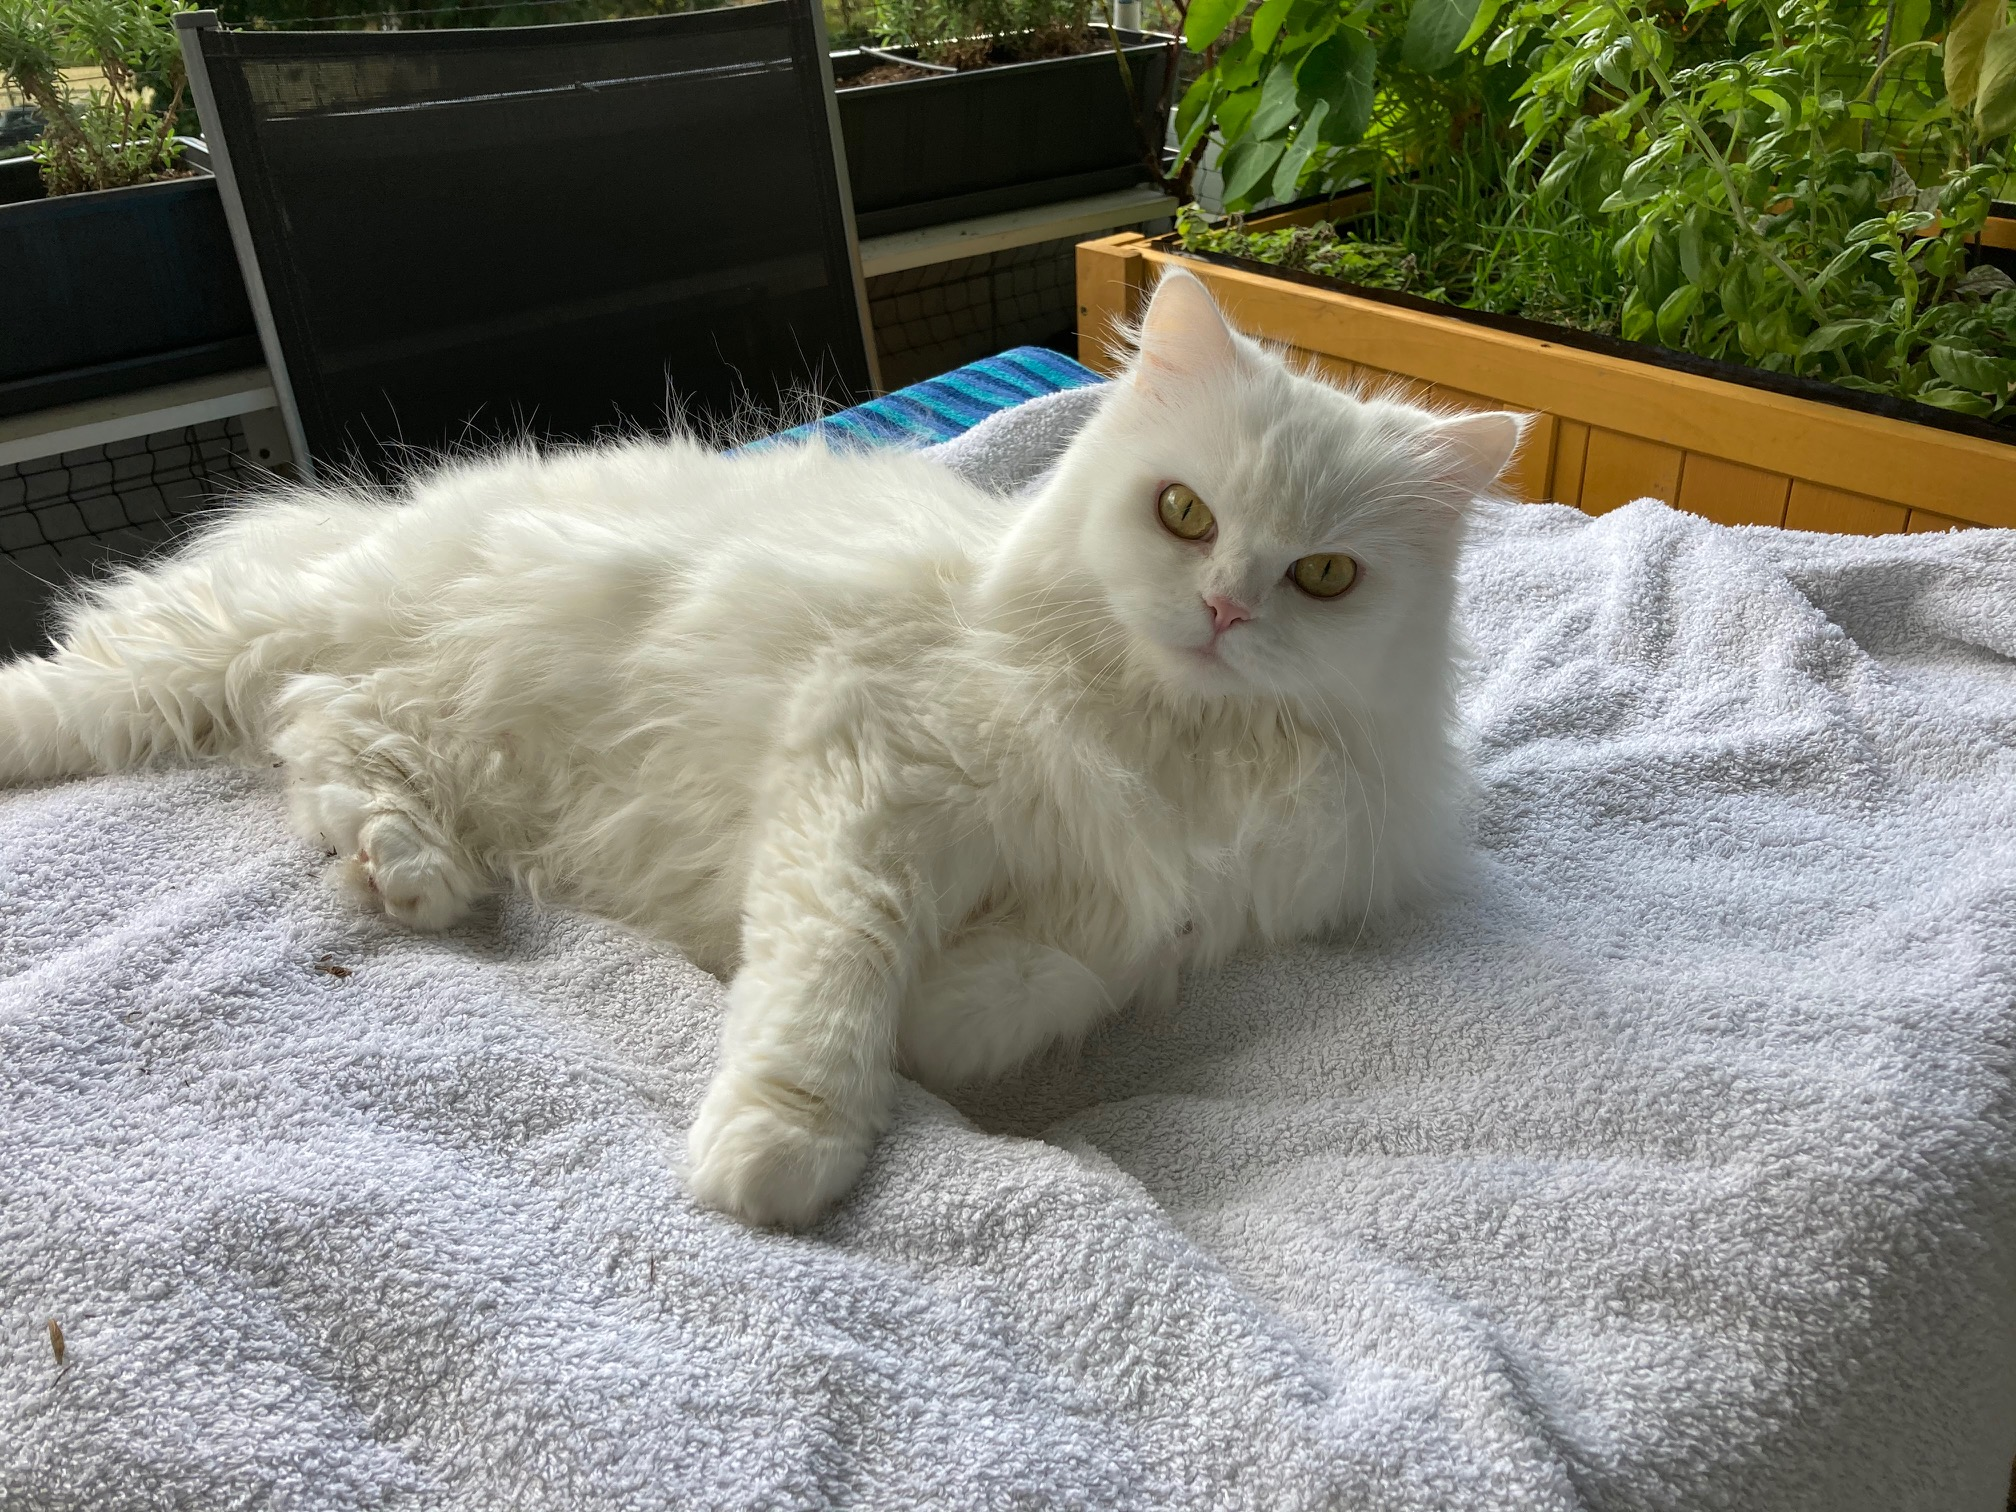
\includegraphics[width=\textwidth]{Katze1}


\end{frame}

\begin{frame}
\frametitle{Bilder}


\includegraphics[width=\textwidth]{Katze}

\end{frame}

\begin{frame}
\frametitle{Bilder}

\begin{columns}
\begin{column}{0.5\textwidth}

\includegraphics[width=\textwidth]{Katze}
\end{column}
\begin{column}{0.5\textwidth}
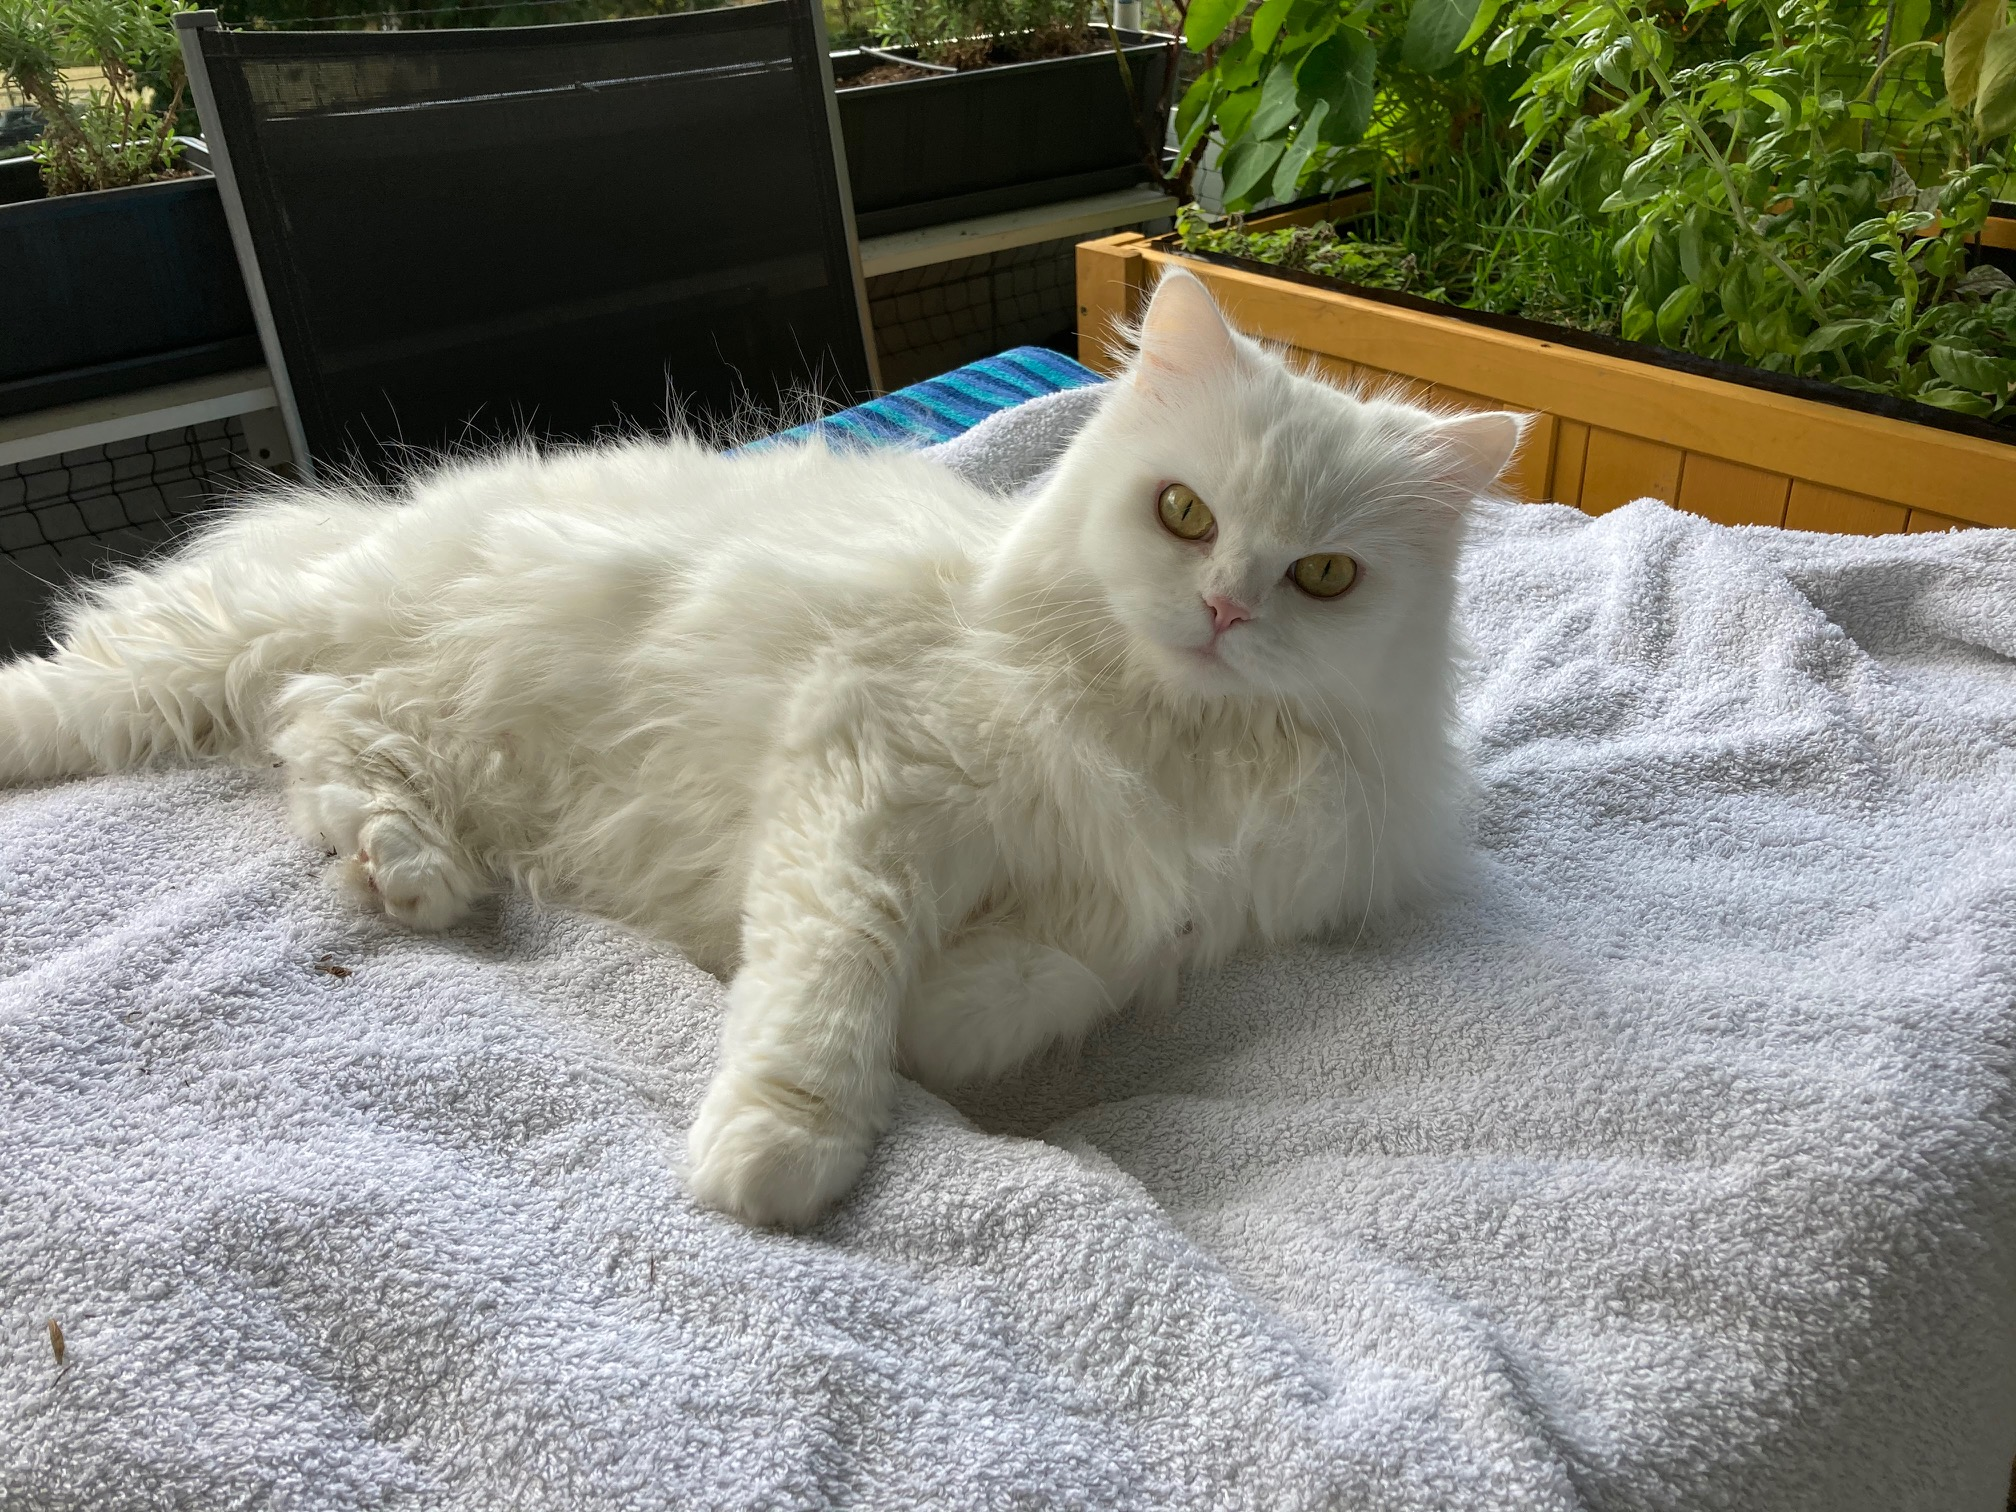
\includegraphics[width=\textwidth]{Katze1}
\end{column}
\end{columns}

\end{frame}

\begin{frame}
\frametitle{Bilder}

\begin{columns}
\begin{column}{0.33\textwidth}
\begin{itemize}
	\item 
	\item 
	\item 
	\item 
	\item 
	\item 
	\end{itemize}
\end{column}
\begin{column}{0.33\textwidth}
\begin{itemize}
	\item 
	\item 
	\item 
	\item 
	\item 
	\item 
	\end{itemize}
\end{column}
\begin{column}{0.33\textwidth}
\begin{itemize}
	\item 
	\item 
	\item 
	\item 
	\item 
	\item 
	\end{itemize}
\end{column}
\end{columns}
\end{frame}

\begin{frame}
\frametitle{Mathe}

\(a+b=c\)

\[-\frac{p}{2} \pm \sqrt{ \left(\frac{p}{2}\right)^2 -q  }\]

\scalebox{5}{\rotatebox{45}{Hallo DLR}}

\end{frame}

\begin{frame}
\frametitle{}

\begin{tabular}{|l|c|r|p{4cm}|} \hline
Spalte 1 & Spalte 2 & Spalte 3 & Spalte 4 \\ \hline
\end{tabular}

\end{frame}


\end{document}